\hypertarget{ch2}{%
\chapter{Physiographic Controls on midwinter snowpack metrics in Sierra Nevada, CA}\label{ch2}}

%==============================================================================
%==============================================================================
%==============================================================================

\hypertarget{ch1-abstract}{\section{Abstract}\label{ch1-abstract}}


%==============================================================================
%==============================================================================
%==============================================================================
\hypertarget{ch1-intro}{\section{Introduction}\label{ch1-intro}}


Water resource management plans in the western US (WUS) are formulated around the assumption that the timing and magnitude of spring snowmelt is stable within the bounds of the interannual variability \citep{livnehDroughtLessPredictable2020}. Climate warming is affecting the stationarity of different processes in the hydrologic cycle all over the world \citep{millyStationarityDeadWhither2008}. In WUS, this means more cold season precipitation falling as rain, and warmer winter temperatures causing midseason melt.


-	On cloudy days, there’s little difference in CS insolation between aspect (cite). 


- hydroclimatic changes are driving increases in fire frequency and intensity \citep{abatzoglouImpactAnthropogenicClimate2016}, air temperatures (Hamlet & Lettenmaier, 2007), midwinter dry spells \citep{hatchettMidwinterDrySpells2023}, could significantly impact society (cite). 

 
Warming temperatures have affected both the accumulation (cite) and ablation (cite) of mountain snowpack, which in turn. The Sierra Nevada is especially susceptible to these changes because its location is in the midlatitudes, where many of the catchments are low to mid-altitude basins, and small increases in temperature could push temperatures above 0 °C ore frequently \cite{gergelEffectsClimateChange2017}. These warming temperatures will affect both precipitation phase partitioning from snow to rain \citep{knowlesTrendsSnowfallRainfall2006}, which will decrease both snowfall amounts and snowpack cold content \citep{harpoldChangesSnowpackAccumulation2012a}. \cite{nolinMappingRiskSnow2006} characterized this type of snow as "at-risk" or snow with the highest potential of being affected by warming temperatures. 

Past studies have leveraged in situ data and models to evaluate snowpack metric trends \citep{clowChangesTimingSnowmelt2010,haleRecentDecreasesSnow2023,harpoldChangesSnowpackAccumulation2012a, moteDECLININGMOUNTAINSNOWPACK2005, moteDramaticDeclinesSnowpack2018, musselmanWinterMeltTrends2021} and the physical mechanisms that govern snowpack snow accumulation and ablation \citep{harpoldHumidityDeterminesSnowpack2018}. Snow pillows cover less than 1 \% of the land area and are limited to mainly mid-elevation flat forest cuts \citep{guan20102011Snow2013}, and macroscale hydrologic models like Variable Infiltration Capacity (VIC) \citep{liangSimpleHydrologicallyBased1994} have resolutions on the scale of kilometers — neither are well-suited for understanding snowpack patterns in complex topography. These physiographic factors impact the local energy balance dynamics, which govern the accumulation and ablation of the snowpack. \cite{musselmanWinterMeltTrends2021} notes the importance of understanding physiographic relationships of snowpack metrics and climatology; therefore, allowing a grasp of how these areas will change (***rework***). \cite{pomeroyVariationSurfaceEnergetics2003} used in situ meteorologic instrumentation setup slope normal, instead of the traditional gravimetric orientation, and found marked differences in incoming shortwave radiation (SW$_{in}$) and ablation rates on south and north facing slopes (**rework**).
-paragraph on snowpack metrics: what are they, why are they important, cite (Nolin et al., 2021)

Previous studies characterized snowpack metrics with respect to physiography. \cite{trujilloSnowpackRegimesWestern2014} used SNOTEL data over the WUS to quantify specific snowpack regimes. \cite{tennantRegionalSensitivitiesSeasonal2017} 

 - What is our, “In this study we…” statement?? \

To better understand how snowpack will react to warming temperatures, we must quantify the physiographic controls on hydrologically important snowpack metrics. Here, we utilize the Sierra Nevada Snow Reanalysis (SNSR), a 90 m spatiotemporally continuous SWE data set from 1985–2016 (32 years), for a comparison of how snowpack metrics change with physiography, specifically aspect and elevation. We analyze three common snowpack metrics: max SWE (MSWE), day of max SWE (DOM), fraction of snow ablation before 1 April (FM) (Musselman et al., 2021), and amount of snow ablation (MWA). We then compare these metrics against annual temperature and a clear sky shortwave radiation (herein SWin) and perform a Spearman’s Rho (SR) (Yue et al., 2002).

ANNE NOTES
- it is key to disaggregate by physiographic parameters which serve as key controls on snowpack energy balance, thus we focus the effects slope and aspect on key snow metrics. \

-info on blowing snow and redistribution
- While detection of monotonic trend is useful for understanding that a given metric is changing, understanding the physical mechanism (i.e., temperature, SW, LW) driving that change illuminates 
-	How does elevation impact SWE, snowfall? How does landscape? \

-	What about slope and aspect? \citep{dozierRevisitingTopographicHorizons2022, dozierApproachEnergyBalance1979} \

-	Why is FM greater lower elevations: rain-snow partitioning/storm temperature \citep{huWidespreadWarmingTrends2020} warmer (temps), \

-	From Musselman: “To explain the elevation-dependent trends and assess whether the observed dynamics are captured in models are beyond the scope of this paper. More generally, an increased understanding of the climatological and physiographical dependencies of snowpack sensitivities to anthropogenic climate warming is needed.” \

-	(A. A. Harpold \& Brooks, 2018) “The observation that seasonal snow cover in the western United States exists across a mean winter temperature range of greater than 12 °C, including multiple locations with mean winter temperatures greater than 0 °C (Fig. 4), highlights the importance of other energy fluxes in controlling snowpack response to climate change.” \

-	While many past studies have leveraged in situ data to evaluate both trends and the physical mechanisms that govern snowpack accumulation and ablation, none have addressed how physiographic variables (e.g. slope and aspect) impact these due to data deficiencies. \

 


%==============================================================================
\hypertarget{ch2-methods}{\section{Methods}\label{ch2-methods}}
\hypertarget{ch2-methods}{\subsection{Study Area}\label{ch2-methods}}

%f12
\begin{figure*}[t]
\centering
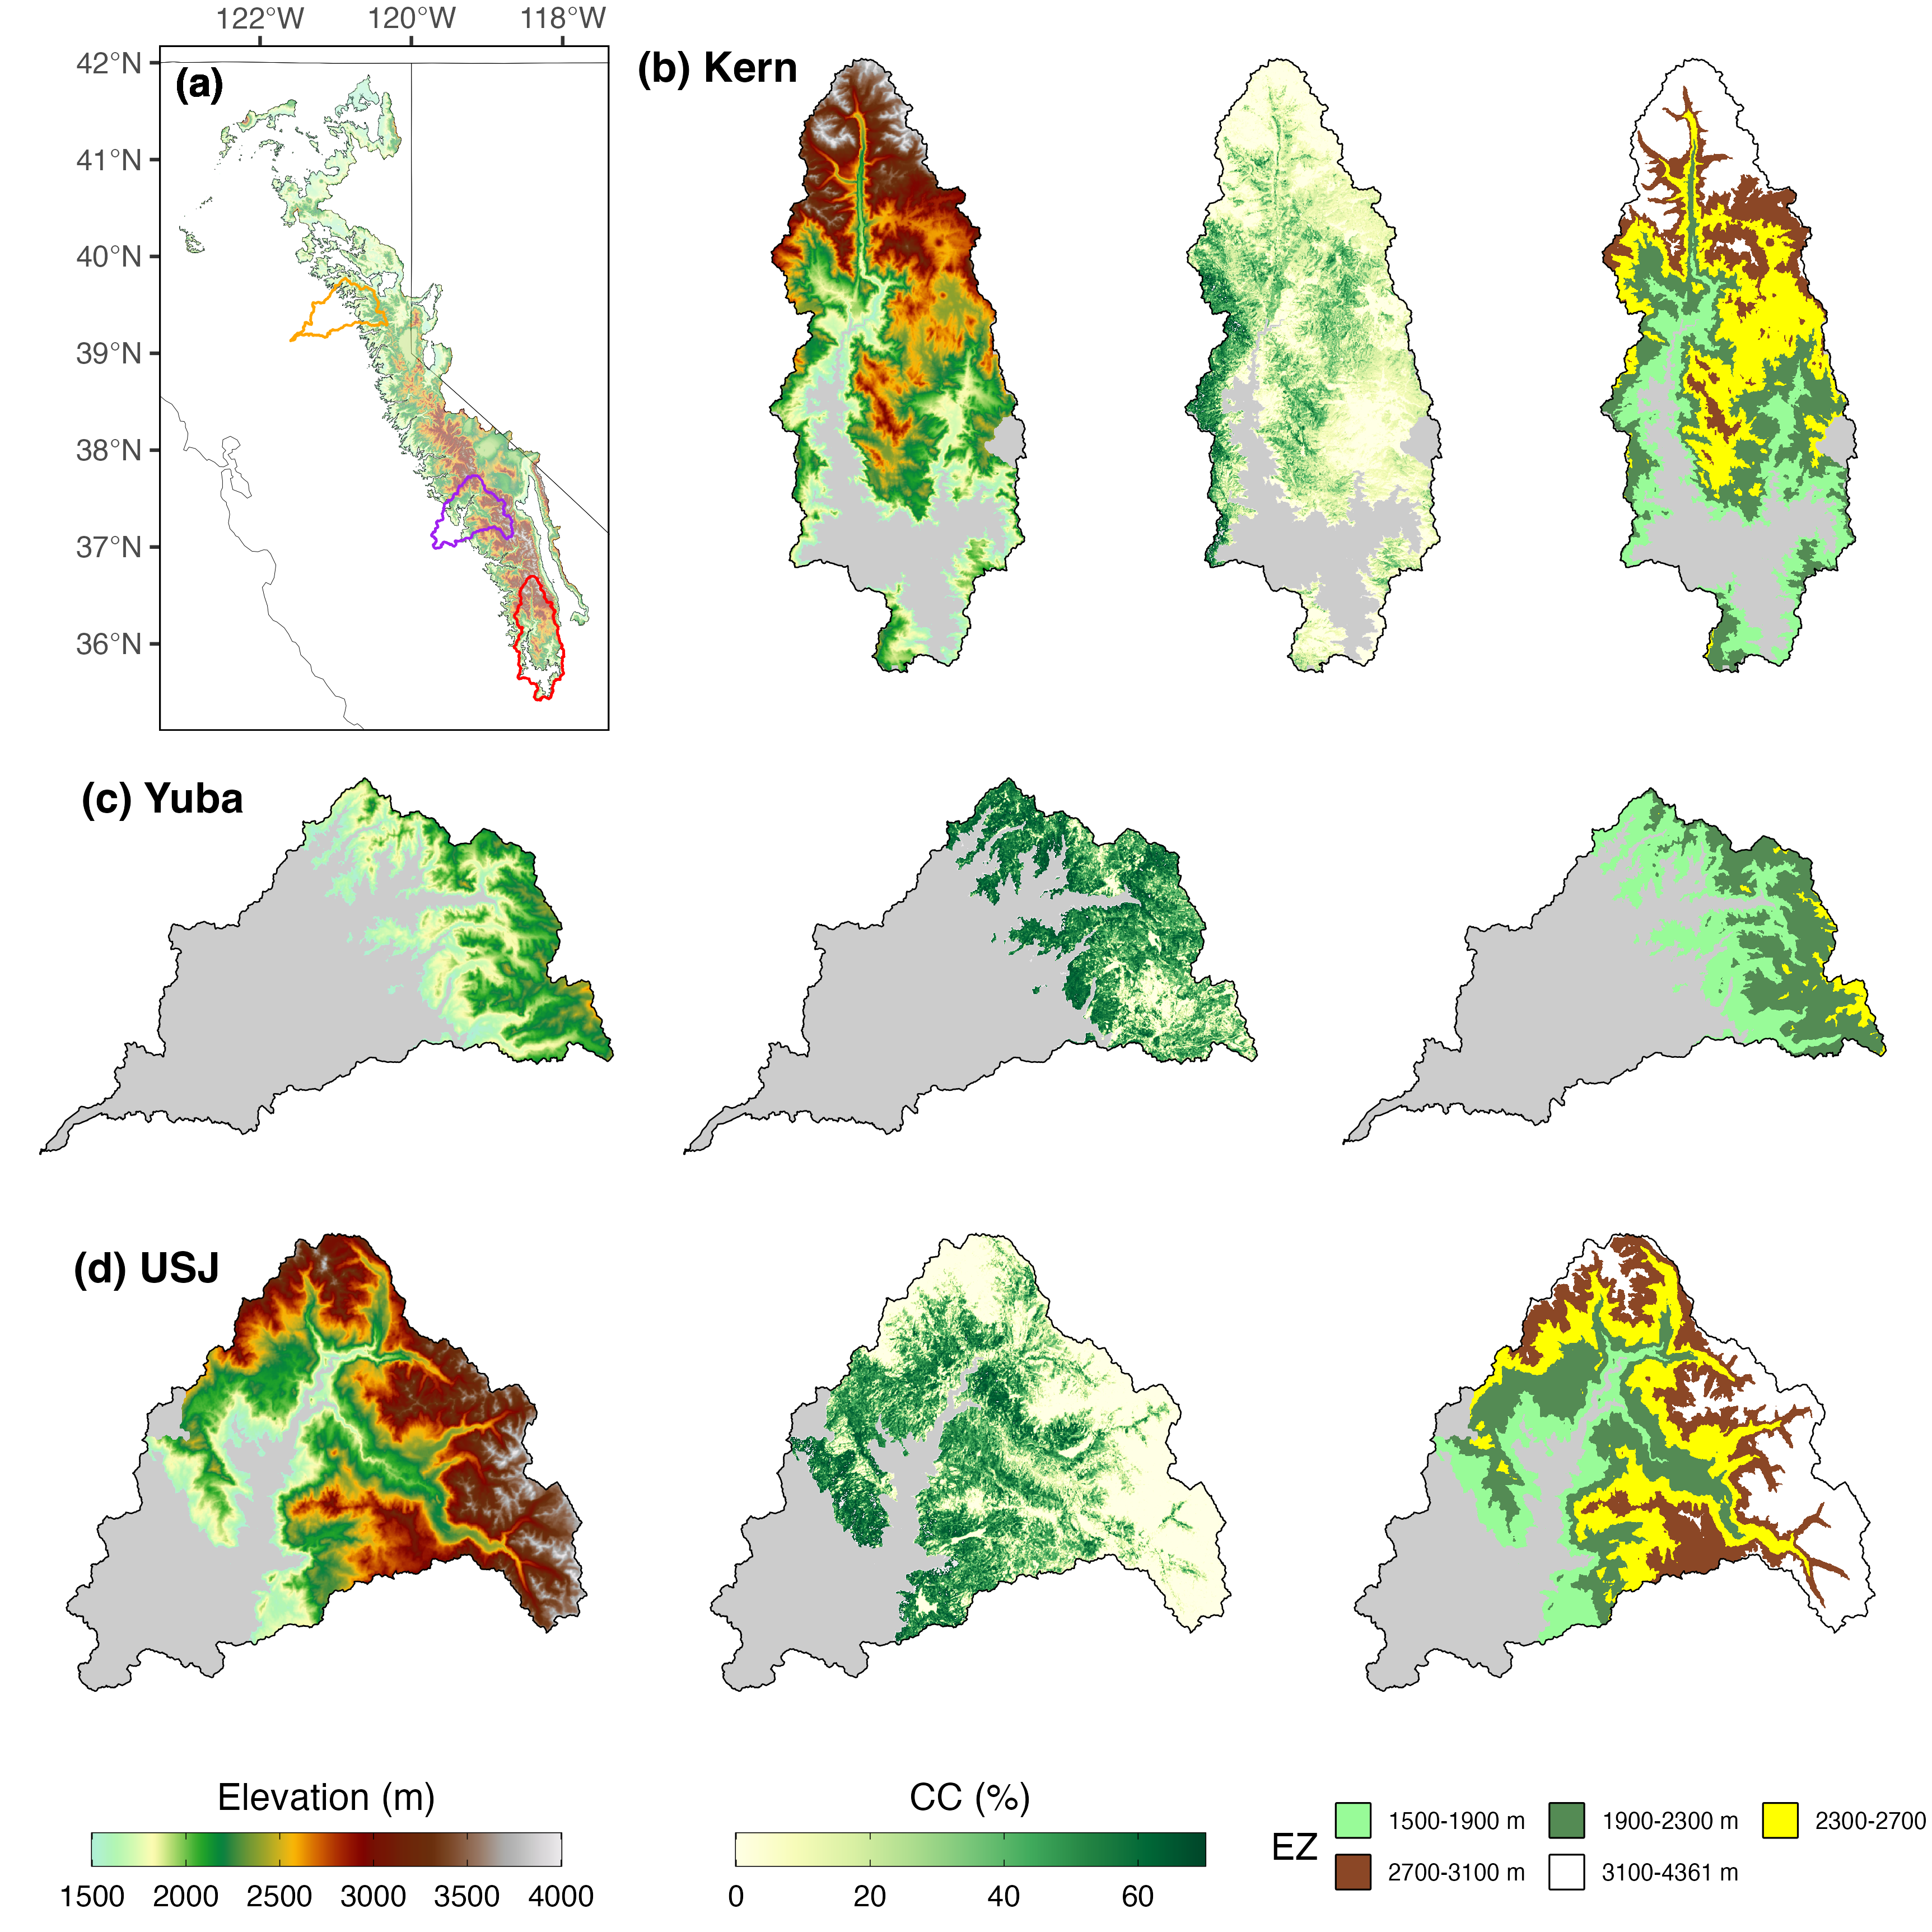
\includegraphics[width=14cm]{figures/ch2_figs/kuy_study_area_v2.png}
\caption{\textbf{(a)} The full extent of the SNSR study domain with Yuba (orange), USJ (purple), and Kern (red) basins shown. The DEM, canopy cover (\%), and elvation zones (EZ) for the three study basins:  \textbf{(b)}~Kern, \textbf{(c)}~Yuba, \textbf{(d)}~USJ.}
\end{figure*}

%==============================================================================
%==============================================================================
%==============================================================================
\hypertarget{ch2-results}{\section{Results}\label{ch2-results}}



%==============================================================================
%==============================================================================
%==============================================================================
\hypertarget{ch2-discussion}{\section{Discussion}\label{ch2-discussion}}


Discussion:
-	-warmer temps increase rate of snow metamorphism (grain growth), increase temp gradients within snowpack (and snowpack and atm), and further increase rate. (Colbeck, Jennings). Larger grain size amplifies the absorption of shorwate (wiscomb and warren, 1980, warren 1980). Midwinter ablation increases the concentration of any light absorbing impurities that may be on the surface (hatchet, gleason, skiles/painter). Hatchet et al. document the increase frequence and length of mid winter dry spells in the sierras. 

The gridMET SRAD data shows both an elevational and latiditunal gradident in values. Our CS insolation model does not account for these variations, and would likely amplify the findings presented herin.

However, the SNSR doesn’t directly address the secondary radiativate forcing, therefore we effect of aspect on snowmelt processes would be amplified.

%==============================================================================
%==============================================================================
%==============================================================================
\hypertarget{ch2-conclusions}{\section{Conclusions}\label{ch2-conclusions}}

\bibliographystyle{apalike}
\setstretch{1}
\bibliography{ch2.bib}
\setstretch{1.5}
